% Very simple template for lab reports. Most common packages are already included.
\documentclass[a4paper, 11pt]{article}
\usepackage[utf8]{inputenc} % Change according your file encoding
\usepackage{graphicx}
\usepackage{url}

%opening
\title{Distributed Systems, Advanced Course \\ 
		Project Report}
\author{KTH Royal Institute of Technology \\ 
	School of Information and Communication Technology \\
	Student:Fanti Machmount Al Samisti (fmas@kth.se) \\
	Student:Pradeep Perris (weherage@kth.se)}
\date{\today{}}

\begin{document}

\maketitle

\tableofcontents

\clearpage

\section{Introduction}

\textit{The goal of this project is to design and implement a distributed key-value store in Kompics. We have used well known distrubuted abstraction model to achive this task: }

Our model employs a (static) membership protocol. Data is partisioned using a Hashing function and replicated within each membership nodes. The data consitency among the replicas during in both reads and updates are achived with (N,N) Atomic Register.

\section{Design Overview}

\subsection{System Component}
The following figure depicts the overall design of the system.

{\centering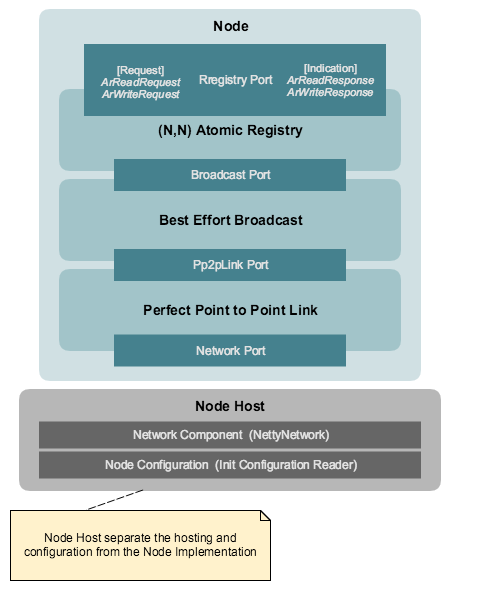
\includegraphics[scale = 0.8]{./images/design_overview.png}\par}

\subsection{Node Toplogy}
{\centering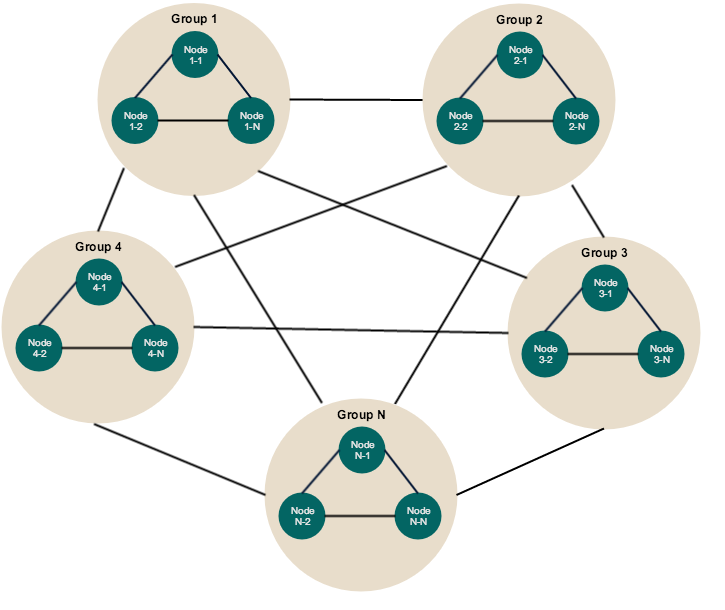
\includegraphics[scale = 0.6]{./images/node_setup.png}\par}

\section{System Abstraction and Implmentation}
\textit{The report should not be too long ($\approx$
	2-3 pages).}

\subsection{Perfect Point to Point Link}

\textit{The report should not be too long ($\approx$
	2-3 pages).}

\subsection{Best Effort Broadcast}

\textit{The report should not be too long ($\approx$
	2-3 pages).}

\subsection{(N,N) Atomic Registry}

\textit{The report should not be too long ($\approx$
	2-3 pages).}

\subsection{Reconfiguration}
\textit{The report should not be too long ($\approx$
	2-3 pages).}

\section{System Simulations and Scenarios}
\textit{The report should not be too long ($\approx$
	2-3 pages).}


\section{Conclusions}

\textit{The report should not be too long ($\approx$
  2-3 pages).}

What have you learnt from the problem presented?
Was it useful?


\end{document}
